\documentclass[tikz,border=2pt]{standalone}
\usepackage{amsmath,amssymb}
\usepackage{tikz}
\usetikzlibrary{arrows.meta,positioning}

\begin{document}
% Peano's picture: start at 0 and keep taking the successor; every natural number is reached
% exactly once, and no step ever returns to 0.
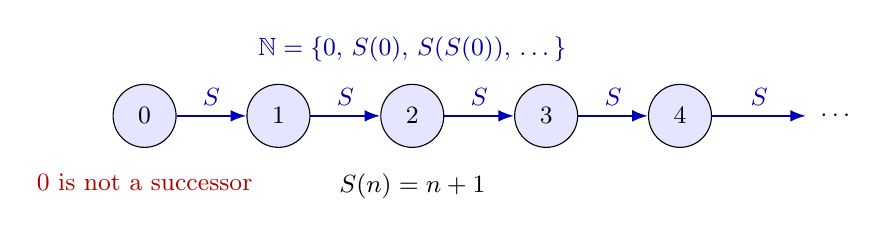
\begin{tikzpicture}[>={Latex[length=2mm]}, every node/.style={font=\small}]
	\foreach \i/\l in {0/0, 1/1, 2/2, 3/3, 4/4} {
		\node[draw, circle, fill=blue!10, minimum size=8mm] (n\i) at (1.7*\i,0) {$\l$};
	}
	\node at (8.8,0) {$\cdots$};
	\foreach \i/\j in {0/1, 1/2, 2/3, 3/4} {
		\draw[->, thick, blue!70!black] (n\i) -- node[above] {$S$} (n\j);
	}
	\draw[->, thick, blue!70!black] (n4) -- node[above] {$S$} (8.4,0);
	\node[red!70!black, below=6pt of n0] {$0$ is not a successor};
	\node[below=6pt of n2] {$S(n)=n+1$};
	\node[above=16pt, blue!60!black] at (n2) {$\mathbb{N}=\{0,\,S(0),\,S(S(0)),\,\dots\}$};
\end{tikzpicture}
\end{document}
